\documentclass[french]{article}
\usepackage[T1]{fontenc} % Font enconding
\usepackage[french]{babel} % Input encoding in French
\usepackage{mathtools} % Include math symbols
\usepackage{amsfonts} % Include font for math symbols
\usepackage{amsthm} % Change definition layout
\usepackage{amssymb} % Use aleph and beth symbols
\usepackage{enumitem} % Modern item enumeration
\usepackage{csquotes} % Typeset quoted texts in French correctly
\usepackage[backend=biber]{biblatex} % For bibliography usage
\usepackage{tikz} % Draw pictures and illustrate examples
\addbibresource{references.bib}
\usepackage{hyperref} % Select links in table of contents
\hypersetup{ 
    colorlinks,
    citecolor=blue,
    filecolor=black,
    linkcolor=blue,
    urlcolor=blue, 
}

\theoremstyle{definition}
\newtheorem{definition}[subsubsection]{Définition}

\theoremstyle{plain}
\newtheorem{proposition}[subsubsection]{Proposition}

\newtheorem{theorem}[subsubsection]{Théorème}

\theoremstyle{plain}
\newtheorem{corollary}[subsubsection]{Corollaire}

\theoremstyle{plain}
\newtheorem{lemma}[subsubsection]{Lemme}

\theoremstyle{plain}
\newtheorem{remark}[subsubsection]{Remarque}

\theoremstyle{plain}
\newtheorem*{notation}{Notation}

\title{UE Projet Tutoré : Ensembles de cardinal infini}
\author{Auteur :\\
	Guillaume SALLOUM \\ 
	L2 Mathématiques \\ 
	Avignon Université
	\and
	Enseignant : \\
	Marc ARCOSTANZO \\
	MCF \\
	Avignon Université}
\date{}

\begin{document}

\maketitle
\begin{abstract}
	Nous étudierons quelques propriétés des ensembles de cardinal infini. 
	Dans un premier temps nous établirons l'existence d'ensembles infinis et indénombrables, en prouvant l'indénombrabilité de \( \mathbb{R} \) à l'aide de l'argument diagnonal de Cantor. 
	Nous construirons ensuite les ordinaux, qui nous permettrons d'aborder très brièvement l'étude des cardinaux infinis. 
	
	Enfin, nous citerons quelques applications de la formalisation des ordinaux.
	Dans tout ce qui suit, on se place dans le modèle axiomatique ZFC où l'on précisera quand on utilise l'axiome du choix, noté AC. 
\end{abstract}


\tableofcontents
\clearpage
\section{Ensembles infinis et dénombrabilité}
\subsection{Bijections et dénombrabilité}

On rappelle des propriétés utilisées dans toute la suite pour comparer deux ensembles entre eux.

\begin{definition}[Ensemble fini]
	Soit \( E \) un ensemble.
	\( E \) est dit fini s'il est vide ou en bijection avec un sous-ensemble de \( \mathbb{N} \) de la forme \( \{1, 2, \ldots, n\} \).
\end{definition}

\begin{definition}[Dénombrabilité]
	Soit \( E \) un ensemble. \( E \) est \textit{dénombrable} si et seulement si on peut énumérer successivement tout les éléments de \( E \) :
\begin{equation*}
	E \coloneqq \{e_{1}, e_{2}, \ldots, e_{n}\} 
\end{equation*} 
	Autrement dit, \( E \) est dénombrable s'il est en bijection avec \( \mathbb{N} \). Sinon \( E \) est dit \textit{indénombrable}.
\end{definition}
\begin{definition}[Cardinal d'un ensemble fini]
	Soit \( E \) et \( F \) deux ensembles \textit{finis}.
	Alors E est en bijection avec un intervalle de \( \mathbb{N} \) de la forme \( \{1, 2, \ldots, n\} \) où \textit{n} est le cardinal de \( E \), noté \( |E| \).
	
	\( E \) et \( F \) sont de même cardinal si et seulement si il existe une bijection de \( E \) dans \( F \).
\
\end{definition}

\begin{proposition}[Ensembles dénombrables]
	\( \mathbb{N} \), \( \mathbb{Z} \) et \( \mathbb{Q} \) sont dénombrables. \cite{tao2014analysis}
\end{proposition}
\begin{proof}
	On se base sur la construction axiomatique de Peano des entiers naturels. 
	Soit \( n \in \mathbb{N} \), alors \( S : n \mapsto n+1 \) la fonction successeur qui assigne à chaque entier naturel son successeur montre que l'on peut énumérer \( \mathbb{N} \).
	
	\par Ensuite, une bijection explicite entre \( \mathbb{N} \) et \( \mathbb{-N} \) est donnée par \( f : n \mapsto -n \). Puisque \( \mathbb{Z} = \mathbb{-N} \cup \mathbb{N} \), et que l'union de deux ensembles dénombrables est à nouveau dénombrable, alors \( \mathbb{Z} \) est dénombrable.
	
	\par Soit \( g : \mathbb{Z} \times \mathbb{Z} \setminus \{0\} \mapsto \mathbb{Q} \) telle que \( g(a,b) \coloneqq \frac{a}{b} \). g est bien définie, et on a \( g(\mathbb{Z} \times \mathbb{Z} \setminus \{0\} ) = \mathbb{Q} \). En particulier, le produit cartésien de deux ensembles dénombrables est à nouveau dénombrable, donc \( \mathbb{Q} \) est dénombrable.

\end{proof}

\subsection{Indénombrabilité de l'ensemble des réels et implications}

\begin{theorem}[Argument diagonal de Cantor]
	\( \mathbb{R} \) n'est pas en bijection avec \( \mathbb{N} \). \cite{aigner2018proofs} \cite{dehornoy2017théorie}
\end{theorem}
\begin{proof}
	Tout sous-ensemble d'un ensemble dénombrable est \textit{au plus dénombrable} : soit fini soit dénombrable. On se restreint donc à l'intervalle \( ]0,1] \) et on montre qu'il n'est pas en bijection avec \( \mathbb{N} \), ce qui implique le résultat énoncé. \\
	Supposons que \( I = ]0,1] \) est dénombrable, alors \( I = \{i_{1}, i_{2}, \ldots \} \). \\ 
	Chaque \( i_{n} \in I \) admet une représentation décimale infinie de la forme :
	\begin{equation*}
		i_{n} = 0,i_{n1}i_{n2}i_{n3}\ldots 
	\end{equation*}
	où \( i_{nk} \in [\![0,9]\!] \).

	On considère le tableau à double entrée formé avec \( i_{1}, i_{2}, \ldots, i_{n}, \ldots \) 

	Soit \( l_{n} \) le plus petit entier dans \( \{1,2\}\) tel que \( l_{n} \neq i_{nk}\). 

	Alors \( r = 0,r_{1}r_{2}r_{3} \ldots r_{n}\ldots \) admet un indice dans le tableau, par exemple \( r = r_{k} \). Or cela est impossible puique \( r_{k} \neq a_{kk} \).
	
\end{proof}

\begin{center}
	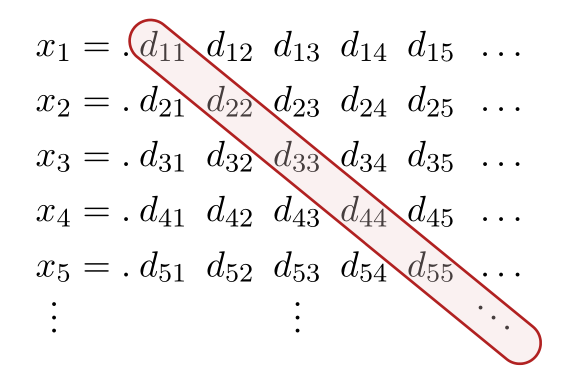
\includegraphics[scale=0.3]{rVEQX.png}
\end{center}
\begin{remark}
	Dans l’illustration ci-dessus, la séquence construite n’est pas exhaustive, on ne peut donc pas dénombrer les réels. On peut aussi montrer que n'importe quelle application \( f : \mathbb{N} \rightarrow [0,1] \) n'est pas surjective, ce qui implique le résultat.
\end{remark}

\begin{theorem}[Cantor, Fraenkel, König]
	L'ensemble \( \mathbb{R}^{2} \coloneqq \mathbb{R} \times \mathbb{R}\) est en bijection avec \( \mathbb{R} \). \cite{aigner2018proofs} 
\end{theorem}
\begin{proof}
	De même que pour le théorème prcédent, on se restreint à établir une bijection entre les paires \( (x,y) \) telles que \( 0 < x,y \le 1 \) sur l'intervalle \( ]0,1] \).
	Soit \( (x,y) \in \mathbb{R}^{2} \) munis de leur représentation décimale infinie :
	\begin{align*}
		x &= 0.r1r2r3 & r4r5 & r6 & &\ldots\\
		y &= 0.r1r2  & r3 & r4 & r5 &\ldots
	\end{align*}

	où l'on sépare chaque décimale de \( x \) et de \( y \) en groupes en prenant à chaque fois la prochaine décimale non nulle (inclusive). Sur un exemple, cela donne :
	\begin{align*}
		x &= 0.3 & 01 && 2 && 007 && 08 & \ldots\\
		y &= 0.009 & 2 && 05 && 1 && 0008 & \ldots
	\end{align*}

	On associe ensuite à cette paire un réel \( r \in ]0,1] \) représenté par le premier groupe de \( x \), le premier groupe de \( y \), le second de \( x \), puis de \( y \) et ainsi de suite.
	Dans l'exemple ci-dessus, cela donne :
	\begin{align*}
		r &= 0.3 & 009 && 01 && 2 && 2 && 05 && 007 && 1 && 08 && 0008
	\end{align*}

	Puisque ni \( x \) ni \( y \) ne forment des suites de décimales composées uniquement de zéros, on trouve qu'il en est de même pour la représentation décimale et non terminalle de r. 
	D'autre part, on peut déduire l'expression de \( x \) et de \( y \) à partir de celle de \( r \) directement, ainsi l'application formée est bijective.
\end{proof}

\begin{remark}
	Il est aussi possible de construire des applications continues, surjectives mais pas injectives entre \( \mathbb{R} \) et \( \mathbb{R}^{2} \) comme le montre l'exemple des courbes de Peano. \cite{peano1890curve}
\end{remark}

\begin{corollary}
	Puisque \( \mathbb{C} \) est isomorphe à \( \mathbb{R}^{2} \), on a \( |\mathbb{C}| = |\mathbb{R}^{2}| = |\mathbb{R}| \).
\end{corollary}

\par On peut étendre la preuve ci-dessus à un nombre fini de coordonnées et obtenir que \( |\mathbb{R}| = |\mathbb{R}^{n}| \) pour \( n \in \mathbb{N} \), résultat obtenu par Cantor en 1878 \cite{kanamori2009set}. 
On établit ainsi l'existence de deux cardinaux infinis distincs : celui de \( \mathbb{N} \) et celui de \( \mathbb{R} \). Avec la proposition suivante, on va voir qu'il en existe une infinité.
\begin{proposition}[théorème de Cantor]
	Soit \( A \) un ensemble. Alors l'ensemble des parties de A et \( A \) ne sont pas en bijection.
\end{proposition} 
\begin{notation}
	On note \( \mathcal{P}(A) \coloneqq \{ I \mid I \subseteq A \}\).	
\end{notation}
\begin{proof}
	Soit \( f : A \rightarrow \mathcal{P}(A) \) quelconque et \( B \coloneqq \{ a \in A \mid a \not\in f(a)\} \). On montre que \( f \) n'est pas surjective. Si \( a \in B \), alors \( a \in B \setminus f(a) \) donc \( f(a) \neq B \). Si \( a \not\in B\) alors \( a \in f(a) \setminus B \) donc \( f(a) \neq B \). D'où \( B \) n'est pas dans l'ensemble image de \( f \), et \( f \) n'est pas surjective.
\end{proof}
\begin{corollary}[Infinité d'infinis]
	Les ensembles \( \mathbb{N}, \mathcal{P}(\mathbb{N}), \mathcal{P}(\mathcal{P}(\mathbb{N})), \ldots \) sont deux à deux non en bijection.
\end{corollary}

D'après l'argument diagonal de Cantor on obtient \( |\mathbb{R}| > |\mathbb{N}| \), ce qui soulève la question de \textit{l'hypothèse du continu} : tout sous-ensemble infini de \( \mathbb{R} \) est-il soit en bijection avec \( \mathbb{N} \), ou avec \( \mathbb{R} \)? Cette question célèbre a notemment motivé le développement de la théorie des ensembles.

\begin{remark}
	On pourra se référer au chapitre 3 partie 2 pour une formulation rigourseuse de l’hypothèse du continu. 
\end{remark}

\clearpage
\section{Ordinaux}

Dans ce chapitre et le suivant, on se basera principalement sur \cite{dehornoy2017théorie}. Les ordinaux constituent une extension de l'arithmétique des entiers naturels et permettent de dénombrer en préservant la propriété de bon ordre. Ils serviront de base à la construction des cardinaux infinis. 
\subsection{Construction des ordinaux} 

\begin{definition}[Bon ordre]
	Soit \( (E,\le) \) un ensemble muni d'une relation d'ordre totale. \( \le \) est un bon ordre si toute partie non vide de \( E \) posséde un élément minimal par rapport à \( \le \). Dans ce cas on appelle \( (E,\le) \) un ensemble \textit{bien ordonné}.	
\end{definition}

\begin{definition}[Segment initial]
	Si \( (E,\le) \) est un ensemble bien ordonné et \( y \in E\), on appelle \textit{segment initial} de \( (E,\le) \) déterminé par \( y \) l'ensemble suivant :
	\begin{equation*}
		Init(y) \coloneqq \{ x \in E \mid x \le y \}
	\end{equation*}
\end{definition}

\begin{proposition}[Comparaison des bons ordres]
	Soit \( (A,\le) \) et \( (B,\preceq) \) deux ensembles bien ordonnées. Alors on a l'un des cas suivants :
	\begin{enumerate}[label = (\roman*)]
		\item \( (A,<) \) et \( (B,\preceq) \) sont isomorphes;
		\item \( (A,<) \) est isomorphe à un segment initial de \( (B,\preceq) \)
		\item \( (B,\preceq) \) est isomorphe à un segment initial de \( (A,<) \)
	\end{enumerate}
\end{proposition}
\begin{proof}[Idée générale de la démonstration]
	On définit une application :
	\begin{align*}
		F : A &\rightarrow B \\
		a &\mapsto F(a) = b \\
			       &\Leftrightarrow \text{Init(a) est isomorphe à Init(b)}
	\end{align*}
	On montre que F est strictement croissante et que le domaine de F est clos par minorant dans \( (A,<) \). Réciproquement, on montre que l'image de F est close par minorant dans \( (B,\preceq) \) pour obtenir que F est un isomorphisme de son domaine sur son image.
\end{proof}
\begin{definition}[Ensemble transitif]
	Soit \( E \) un ensemble quelconque. E est \textit{transitif} si tout les éléments d'éléments de \( E \) sont des éléments de \( E \). En d'autres termes :
	\begin{equation}\label{eq:Tr} \tag{Tr}
		x \in a \in E \implies x \in E 
	\end{equation}

	\( E \) est donc un \textit{ensemble pur} particulier.  \cite{nlab:pure_set} \cite{nlab:transitive_set} 
\end{definition}

\begin{lemma}[Stabilité par opérations ensemblistes]
	\begin{enumerate}[label = (\roman*)]
		\item \( \emptyset \) est transitif ;
		\item Si \( E \) est transitif, alors \( E \cap \{E\} \), \( \bigcup E \) et \( \mathcal{P}(E) \) le sont aussi ;
		\item Toute réunion ou intersection d'ensemble transitifs est transitive
	\end{enumerate}
\end{lemma}

\begin{proof}
	\begin{enumerate}[label = (\roman*)]
		\item Comme \( \emptyset \) n'a pas d'éléments \eqref{eq:Tr} est vérifiée.
		\item On suppose que \( E \) est transitif. Si \( x \in e \in E \cup \{E\} \) alors \( x \) est dans \( E \) ou \( x = E \). Dans les deux cas \( x \in E \) donc à fortiori \( x \in E \cup \{E\} \). Donc \( E \cup \{E\} \) est transitif.

			Supposons \( x \in E \in \mathcal{P}(E) \), alors \( x \in e \subseteq E \) et donc \( x \in E \). D'après \eqref{eq:Tr}, \( x \subseteq E \) donc \( x \subseteq \mathcal{P}(E)\). Donc \( \mathcal{P}(E) \) est transitif.

			Supposons \( x \in E \in \bigcup E \). Il existe \( y \in E \) tel que \( x \in y \in E \), donc \( x \in E \) puisque \( E \) est transitif, et \( x \in \bigcup E \). Donc \( \bigcup E \) est transitif.
		\item Soit \( (E_{i})_{i \in I} \) une famille d'ensembles transitifs. Supposons \( x \in a \in \bigcup_{i\in I} A_{i} \). Il existe donc \( i \) vérifiant \( x \in a \in A_{i} \), donc \( x \in A_{i} \) par hypothèse, et aussi \( x \in \bigcup_{i \in I}\). Donc \( \bigcup_{i \in I} A_{i} \) est transitif. On utilise le même raisonnement avec \( \bigcap_{i \in I} A_{i} \) pour obtenir le résultat énoncé.
	\end{enumerate}
\end{proof}

\begin{definition}[Ordinal]
	Un ensemble \( \alpha \) est un ordinal si \( \alpha \) est transitif et que la restriction de \( \in  \) à \( \alpha \) notée \( \in_{|\alpha} \) est un bon ordre strict.
\end{definition}

\begin{definition}[Caractérisation des ordinaux]
	Un ensemble \( \alpha \) est un ordinal si on a :
	\begin{enumerate}[label = (\roman*)]
		\item \( \forall x \in \alpha \), \( x \subseteq \alpha \) ;
		\item \( \forall x \in \alpha \), \( x \not\in x \) ;
		\item \( \forall x, y, z \in \alpha \), si \( x \in y \) et \( y \in z \), alors \( x \in z \) ;
		\item \( \forall I \subseteq \alpha \), \( I \neq \emptyset \), \( \exists x \in \alpha \) tel que \( x \in y \) pour tout \( y \in I \) avec \( x \neq y \).
	\end{enumerate}
\end{definition}

\subsection{Arithmétique des ordinaux}

\par Puisque les ordinaux forment un cas particulier d'ensembles transitifs, les ordinaux sont stables par union et par intersection d'après le Lemme 2.1.5. On peut donc construire une infinité d'ordinaux.

\begin{definition}[Successeur]
	Soit \( E \) un ensemble et \( S(E) \coloneqq E \cup \{E\} \). Pour \( n \in \mathbb{N} \), on note \( \underline{n} \) l'ordinal \( S^{n}(\emptyset) \).
\end{definition}

\begin{description}
	\item \( \underline{0} = \emptyset \),
	\item \( \underline{1} = S(\underline{0}) = \{\underline{0}\} \),
	\item \( \underline{2} = S(\underline{1}) = \underline{1} \cup  \{\underline{1}\} = \{\underline{0}\} \cup \{\underline{1}\} = \{\underline{0}, \underline{1}\},  etc.\)
\end{description}

On montre à partir de cette définition qu'un ordinal \( \underline{n} \) possède exactement \( n \) éléments.
\begin{proposition}[Ordinaux \underline{n}]
	Soit \( n \in \mathbb{N} \). L'ordinal \( \underline{n} \) admet exactement \( n \) éléments qui sont les ordinaux \( \underline{k} \) pour \( k < n \).
\end{proposition}
\begin{proof}
	On raisonne par récurrence sur \( n \). 
	
	L'ordinal \( \underline{0} \) n'admet aucun élément par définition.
	On suppose \( n > 0 \), et on pose \( m \coloneqq n - 1 \). Puisque \( \underline{n} = \underline{m} \cup \{\underline{m}\} \), par hypothèse n est formé des \( m \) ordinaux \( \underline{k} \) où \( k < m \) et de \( \{\underline{m}\} \). Or \( \{\underline{m}\} \) est transitif, donc n'est pas dans \( \underline{m} \). D'où \( \underline{n} \) a \( n \) éléments qui sont les ordinaux \( \underline{k} \) avec \( k < n \).
\end{proof}

\begin{proposition}[Borne inférieure et bon ordre]
	Tout ensemble non vide d'ordinaux \( E\) admet un minorant \( \bigcap E \).
\end{proposition}
\begin{proof}
	On pose \( \alpha \coloneqq \bigcap E \). Pour tout \( \beta \) dans \( E \) on a \( \alpha \in \beta \) donc \( \alpha \le \beta \). Si \( \alpha < \beta \) alors \( \alpha \in \bigcap E \) et \( \alpha \in \alpha \) ce qui contredit la définition 2.1.7. Donc on doit avoir \( \alpha = \beta \) où \( \alpha \) est le plus petit élément de \( E \).
\end{proof}
\begin{proposition}[Borne supérieure]
	Un ensemble d'ordinaux \( E \) possède une borne supérieure \( \bigcup E \). 
\end{proposition}
\begin{proof}
	Soit \( e \coloneqq \bigcup E \). Les éléments de \( E \) sont transitifs donc \( e \) est transitif. De plus \( \forall \alpha, \beta, \gamma \in E \), par propriétés des ensembles transitifs \( \alpha \notin \alpha  \) et si \( \alpha \in \beta \in \gamma \) alors \( \alpha \in \gamma \). Donc la relation \( \in_{|e} \) est un bon ordre strict. D'où \( e \) est un ordinal.

	Soit \( X \in \bigcup E \) non vide et \( \alpha \coloneqq \bigcap X \). Alors \( \alpha \) est un ordinal qui minore \( X \) d'après la proposition 2.2.3. Cela implique que pour tout \( \beta \in X \) distincts de \( \alpha \) on a \( \alpha \in \beta \). 

	Pour tout \( \alpha \in E \) on a \( \alpha \subseteq e \), donc \( \alpha \le e \). Si \( \beta \) est un minorant strict de \( e \) on a \( \beta < e \) et \( \beta \in \bigcup E \). On a donc un \( \alpha \) dans la réunion tel que \( \beta \in \alpha \) et \( \beta < \alpha \) où \( \beta \) n'est pas un majorant de \( E \). Ainsi \( e \) est le plus petit majorant de \( E \).
\end{proof}

\par On cite un résultat simialire au paradoxe de Russell sur les ensembles : on ne peut pas construire un ensemble qui contient tout les ordinaux (pas seulement les ordinaux \( \underline{n} \)).

\begin{proposition}[Paradoxe de Burlati-Forti]
	Il n'existe pas d'ensemble contenant tout les ordinaux.
\end{proposition}
\begin{proof}
	On raisonne par l'absurde en supposant qu'il existe un ensemble \( \Omega \) contenant tout les ordinaux.
	
	Alors \( \bigcup \Omega \) est un ordinal qui vérifie : \( \forall \alpha \in \Omega, \alpha \le \bigcup \Omega \). 

	Donc \( \bigcup\Omega < S(\bigcup\Omega) \le \bigcup\Omega \), ce qui implique \( \bigcup\Omega \in \bigcup\Omega \), or cela contredit 2.1.7.
\end{proof}

\begin{remark}
	Par conséquent, les ordinaux forment une \textit{classe propre}, c'est-à-dire une classe qui n'est pas un ensemble, terminologie utilisée dans la théorie des ensembles de von-Neumann–Bernays–Gödel (NBG). On note en général \textbf{Ord} la classe des ordinaux. 
	Dans ZF, les classes ne sont pas définies de manière formelle, et on doit expliciter une formule ensembliste pour spécifier la classe (voir la section sur les cardinaux ci-dessous pour un exemple). 

\end{remark}
\par On distingue désormais deux familles d'ordinaux.
\begin{definition}[Ordinal successeur, limite]
	Soit \( \alpha \) un ordinal non nul. \( \alpha \) est dit successeur s'il existe \( \beta \) vérifiant \( \alpha = S(\beta) \), et limite si on a \( \alpha = \bigcup \alpha \).
\end{definition}

\begin{definition}[Ensemble récurrent]
	Un ensemble est dit récurrent s'il contient \( \emptyset \) et est clos par l'application \( S : x \mapsto x \cup \{x\} \).
\end{definition}
\begin{definition}[Ordinal omega]
	On définit l'ordinal \( \omega \) comme le plus petit ordinal récurrent.
\end{definition}

\begin{corollary}
	Pour tout \( n \in \mathbb{N} \), on a \( \underline{n} < \omega \).
\end{corollary}

\begin{proof}
	L'ensemble vide n'est pas récurrent, et on peut montrer par récurrence qu'aucun ordinal \( \underline{n} \) n'est récurrent.
\end{proof}

\par Par conséquent, on a :
\begin{equation*}
	\omega = \{\underline{0}, \underline{1}, \underline{2}, \ldots\}
\end{equation*}

\par On représente la construction obtenue jusqu'ici : la suite des ordinaux où \( \omega \) est un ordinal limite.
\begin{center}
	\begin{tikzpicture}
	\draw [line width=2pt] (0,0) -- (10,0);
	\foreach \x in {0,1,...,9}
	\filldraw[color=black] (\x,0) circle [radius=2pt] node[below=2ex] {$\underline{\x}$};
	\draw [line width=2pt, dashed] (10,0) -- (11.5,0);
	\draw [line width=2pt, ->] (12,0) -- (16.5,0);
	\filldraw[color=black] (12,0) circle [radius=2pt] node[below=2ex] {$\omega$} node[above=2ex] {fini \( \leftarrow \mid \rightarrow \) infini };
	\filldraw[color=black] (13,0) circle [radius=2pt] node[below=2ex] {$S(\omega)$};
	\filldraw[color=black] (14,0) circle [radius=2pt] node[below=2ex] {$S^{2}(\omega)$};
\end{tikzpicture}
\end{center}

\begin{proposition}[Induction ordinale]
	Le principe de récurrence définit sur les entiers peut s'étendre aux ordinaux \( \underline{n} \).
\end{proposition}
\begin{proof}
	On étend le principe de récurrence connu sur \( \mathbb{N} \). La preuve étant plutôt longue, elle ne sera pas exposée ici, le lecteur intéréssé pourra se référer à \cite{dehornoy2017théorie} pour vérifer que cela fonctionne.
\end{proof}

\par Une conséquence importante de ce résultat est un théorème qui servira de base à la construction des cardinaux infinis : on peut exhiber un représentant unique pour chaque ensemble bien ordonné.

\begin{theorem}[Comparaison]
	Tout ensemble bien ordonné \( (E,<) \) est isomorphe à un unique ordinal.
\end{theorem}
\begin{proof}
	Soit \( (E,<) \) un ensemble bien ordonné. 
	
	D'après la Proposition 2.1.3, soit \( (E,<) \) est isomorphe à la suite des ordinaux, soit la suite des ordinaux est isomorphe à un segment initial de \( (E,<) \), ou bien \( (E,<) \) est isomorphe à un segment initial de la suite des ordinaux.

	Or la suite des ordinaux ne forme pas un ensemble d'après le paradoxe de Burlati-Forti, donc il ne reste que le dernier cas. Un segment initial de la suite des ordinaux est un ordinal par transitivité. Par unicité des segments initiaux, l'ordinal obtenu est unique, d'où le résultat. 
\end{proof}

\par Enfin, on peut étendre les opérations d'addition, de multiplication et d'exponentiation des entiers aux ordinaux avec quelques modifications supplémentaires : l'addition et la multiplication ne sont pas commutatives par exemple.

\clearpage
\section{Cardinaux infinis}
\subsection{Definitions et généralités}

\par Avec l'axiome du choix, on peut établir une bijection entre un ensemble et un ordinal.

\begin{remark}
	Dans cette section, nous définirons la suite des cardinaux infinis à l'aide de AC. Cela permet en particulier de conserver l'ordre total sur les cardinaux, puisque AC implique qu'un ordinal est un cardinal. Sans AC, on peut conserver une relation d'ordre partielle, ce qui rend les relations de comparaison entre cardinaux infinis plus complexes à manipuler. On ne développera pas ici cette théorie (voir \cite{jech1973axiom} chapitre 11 p.156 pour une exposition plus complète du sujet).
\end{remark}

\begin{definition}[Cardinal]
	Un cardinal est un ordinal qui n'est en bijection avec aucun ordinal plus petit que lui-même.
\end{definition}

\begin{proposition}[Cardinalité]
	Tout ensemble est en bijection avec un unique cardinal.
\end{proposition}
\begin{proof}	
	\textit{Existence :} D'après le théorème de Zermolo, pour tout ensemble \( E \), il existe un bon ordre \( < \) sur \( E \), et d'après le théorème de comparaison il existe un unique ordinal \( \alpha \) tel que \( (E,<) \) est isomorphe à \( (\alpha,\in) \). Soit \( \kappa \) le plus petit des ordinaux en bijection avec \( \alpha \). Alors \( \kappa \) est un cardinal par construction en bijection avec lui-même. 

	\textit{Unicité : } Soit \( \kappa, \mu \) deux cardinaux distincts. Alors par bon ordre strict l'un des deux est plus grand que l'autre, donc il ne peut pas y avoir de bijection entre les deux.
\end{proof}

\begin{corollary}
	Un cardinal infini est un ordinal limite.
\end{corollary}
\begin{notation}
	On note \( |E| \) l'unique cardinal \( \kappa \) tel que E est en bijection avec \( \kappa \).
\end{notation}

\begin{proof}
	Pour tout ordinal infini \( \alpha \) il existe une bijection de \( \alpha \) sur \( \alpha + 1 \), ce qui donne le résultat. Par exemple, on a \( |\omega + 1| = \omega \). Il est important de mentionner que cette bijection ne préserve pas l'ordre. \cite{gowers2010ordinals}
\end{proof}

\begin{corollary}
	Pout tout ensemble \( E \), on a \( |E| < |\mathcal{P}(E)| \).
\end{corollary}
\begin{proof}
	C'est une conséquence directe du théorème de Cantor.
\end{proof}

\begin{definition}[Successeur, limite]
	Soit \( \kappa \) un cardinal infini. De même que pour les ordinaux, on note \( \kappa^{+} \) le successeur de \( \kappa \) et on appelle \textit{cardinal limite} tout cardinal qui n'est pas un successeur.
\end{definition}

\begin{remark}
	Puisque les ordinaux ne forment pas un ensemble mais une classe propre, il en est de même pour les cardinaux. On peut expliciter que \( \kappa \) est un cardinal avec la formule ensembliste suivante :

	\par \( \kappa \in \textbf{Ord},  \forall{\alpha < \kappa}, \forall{f : \alpha \mapsto \kappa}, \exists{\beta \in \kappa}, \forall{\gamma \in \alpha}, (f(\gamma) \neq \beta) \).

	La classe des cardinaux est notée \textbf{Card}.
\end{remark}

\subsection{Alephs}

\par On énumère désormais les cardinaux infinis à l'aide des résultat suivant.

\begin{lemma}[La suite des cardinaux n'est pas bornée]
	Pour tout ensemble infini \( E \), il existe un plus petit ordinal \( \Theta \) ne s'injectant pas dans \( E \) tel que \( \Theta \) s'injecte dans \( \mathcal{P(\mathcal{P}}(E \times E))\). De plus \( \Theta \) est un cardinal.
\end{lemma}
\begin{proof}[Idée générale de la démonstration]
	On utilise la notion de classe fonctionnelle pour expliciter l'existence de \( \theta \) et prouver le fait que c'est un cardinal. L'argument reposant sur la structure de classe, il ne sera donc pas développé ici, on pourra se référer à \cite{dehornoy2017théorie} pour la démonstration complète.
\end{proof}

\begin{proposition}[Successeur]
	Pour tout cardinal infini \( \kappa \), il existe un plus petit cardinal infini \( \Theta \) tel que \( \kappa < \Theta \).
\end{proposition}
\begin{proof}
	D'après la proposition précédente, \( \Theta \) ne s'injecte pas dans \( \kappa \) et est un cardinal. Tout cardinal \( \mu < \kappa \) s'injecte dans \( \kappa \) donc \( \kappa < \Theta \). Si \( \lambda \) vérifie \( \lambda <  \Theta \) alors \( \lambda \le \kappa \). Donc \( \Theta \) est le plus petit cardinal supérieur à \( \kappa \).  
\end{proof}

\par Ces deux résultats permettent de définir la classe des alephs :
\begin{definition}
Pour tout ordinal \( \alpha \), on note \( \aleph_{\alpha} \) le cardinal infini \textit{aleph alpha} tel que :
	\begin{enumerate}[label = (\roman*) ]
		\item \( \aleph_{0} \coloneqq \omega \);
		\item \( \aleph_{\alpha + 1} \coloneqq \aleph_{\alpha}^{+} \);
		\item \( \aleph_{\lambda} \coloneqq \sup_{\alpha < \lambda} \aleph_{\alpha} \) où \( \lambda \) est un ordinal limite.
	\end{enumerate}
\end{definition}

\begin{proposition}[Enumération canonique]
	Tout cardinal infini \( \kappa \) est un aleph.
\end{proposition}

\begin{proof}
La suite des alephs définie ci-dessus est un suite de cardinaux strictement croissante. On montre par récurrence sur \( \kappa \) qu'il existe un ordinal \( \alpha \) tel que \( \kappa = \aleph_{\alpha} \), c'est-à-dire que la suite des \( \aleph_{\alpha} \) est surjective. \cite{dehornoy2017théorie}.
\end{proof}

\begin{definition}[Hypothèse du continu généralisée (GCH)]
	\begin{equation}\label{eq:GCH1} \tag{GCH1} 
		\forall{\kappa \in \textbf{Card} }, 2^{\kappa} = \kappa^{+}.
	\end{equation}
On peut reformuler cette définition avec les alephs :
	\begin{equation}\label{eq:GCH2} \tag{GCH2}
	\forall{\alpha \in \textbf{Ord}}, 2^{\aleph_{\alpha}} = \aleph_{\alpha+1} 
	\end{equation}
Par exemple, pour \( \aleph_{0} \) cela donne l'hypothèse du continue sur \( \mathbb{R} \) :
	\begin{equation}\label{eq:HC} \tag{HC}
	|\mathbb{R}| = 2^{\aleph_{0}} = \aleph_{1} 
	\end{equation}

\end{definition}

\subsection{Nombres de Beth}

\par Les nombres de Beth forment une autre énumération non-exhaustive des cardinaux infinis. En effet, contrairement aux alephs, tout les cardinaux infinis ne sont pas des nombres de Beth.
\begin{definition}[Nombre de Beth]
	On note \( \beth_{\alpha} \) le \textit{alpha-ième} nombre de Beth, où \( \alpha \) est un ordinal, défini de la manière suivante à l'aide du passage aux parties de \( \mathbb{N} \) :
	\begin{enumerate}[label = (\roman*) ]
		\item \( \beth_{0} \coloneqq \aleph_{0} \);
		\item \( \beth_{\alpha + 1} = 2^{\beth_{\alpha}} \);
		\item \( \beth_{\lambda} = \sup_{\alpha < \lambda} \beth_{\alpha} \) où \( \lambda \) est un ordinal limite.
	\end{enumerate}

	\par On a donc : 

	\( \beth_{0} = |\mathbb{N}| \), \( \beth_{1} = |\mathcal{P}(\mathbb{N})|,\) \( \beth_{2} = |\mathcal{P}(\mathcal{P}(\mathbb{N}))| \), et ainsi de proche en proche.

\end{definition}
\par Si l'hypothèse du continue généralisée est admise, on a : \cite{4301717}
\begin{equation*}
	\forall \alpha \in \textbf{Ord}, \aleph_{\alpha} = \beth_{\alpha}
\end{equation*}

\clearpage

\section{Applications}
\subsection{Applications en Analyse}
\subsubsection{Ensemble image d'une fonction continue sur un compact}

\par La formalisation des ordinaux permet de donner des preuves alternatives à certains problèmes d'analyse. On expose ici une preuve issue de \cite{gowers2010ordinals}.

\begin{proposition}
	L'ensemble image d'une fonction continue sur l'intervalle fermé compact \( [0,1] \) est borné.
\end{proposition}

\begin{proof}
	On montre d'abord que tout les sous-ensembles bien ordonnés de \( [0,1] \) sont dénombrables. Soit \( E_{\alpha} \) un sous-ensemble de \( [0,1] \) bien ordonné indexé par un ordinal \( \alpha \). Alors l'application :
\begin{align*}	
	g : \alpha &\rightarrow E_{\alpha} \\
	x &\mapsto e_{x}
\end{align*}
est un isomorphisme qui préserve l'ordre. Donc pour \( x < y \), il n'y a pas d'élément entre \( e_{x} \) et \( e_{y} \). L'intervalle \( [e_{x},e_{y}] \) contient un nombre fini de rationnels distincts, et on peut en déduire que \( E_{\alpha} \) est dénombrable.

Si f est continue sur \( [0,1] \), il existe \( s > x \) tel que f est bornée sur \( [0,s] \). L'intervalle \( ]x,s] \) contient un nombre fini de rationnels. On définit \( y \) tel que \( e_{y} \) où \( y \) est un ordinal succeseur de x tel que f est bornée sur \( [0,q] \) avec q le premier rationnel successeur. Sinon \( y \) est un ordinal limite où \( e_y = \sup_{x<y} e_{x} \). 

Alors f est bornée jusqu'à \( e_{y} \). Tant que \( y \neq 1 \), cette construction définit un isomorphisme unique qui préserve l'ordre entre \( E_{\alpha} \) et \( [0,1] \).

\end{proof}

\subsubsection{Convergence des suites de Goodstein}

\par Un entier \( n \) peut être décomposé dans la base \( p \geq 2 \) :
\begin{equation*}
	n = p^{n_{1}}.c_{1} + \ldots + p^{n_{k}}.c_{k}
\end{equation*}
Les exposants \( n_{i} \) peuvent être eux aussi exprimés en base \( p \) pour obtenir le développement itéré (ou héréditaire) de \( n \) en base \( p \).

\begin{definition}[Suite de Goodstein]
La suite de Goodstein d'un entier \( m \), notée \( G_{n}(m) \) est définie récursivement :
\begin{enumerate}[label = (\roman*)]
	\item Si \( G_{n}(m) = 0 \), la suite \( G(m) \) est finie de longueur 0
	\item Sinon on écrit \( G_{n}(m) \) en notation héréditaire en base \( n+1 \), puis on remplace \( n+1 \) par \( n+2 \). Puis on soustrait 1 au résultat et on obtient \( G_{n+1}(m) \).
\end{enumerate}
\end{definition}

\begin{proposition}
	Toute suite de Goodstein \( G_{n}(m) \) converge vers 0
\end{proposition}

\begin{proof}[Idée générale de la preuve]
	On construit une suite d'ordinaux \( T_{n}(m) \) strictement décroissante et terminale, qui implique que \( G_{n}(m) \) se termine lorsqu'elle s'annule. \cite{dehornoy2017théorie}
\end{proof}

\subsection{Applications en Théorie des jeux combinatoires}

\par En théorie des jeux combinatoires, on modélise un jeu sans élément aléatoire à deux personnes \( G \) comme une paire ordonnée \( G=(L,R) \) possédant une condition terminale, où \( L \) et \( R \) sont des ensembles, dont les éléments désignent les options que chque joueur possède à une position donnée. Les ordinaux, munis d'une nouvelle opération d'addition et de multiplication, servent à modéliser les tas dans les jeux de Nim. Un tas d'allumettes dans un jeu de Nim est alors appelé \( nimber \), et est un ordinal particulier. 

Il existe une classification des jeux impartiaux d'après Sprague-Grundy, où chque jeu impartial est équivalent à un tas fini dans un jeu de Nim, avec une stratégie triviale de réussite. Mais cela ne rend pas chque jeu impartial facile à analyser, car il faut trouver quel nimber est équivalent au jeu en question. \cite{schleicher2005introduction}

Plus généralement, Conway utilise dans \cite{conway2000onag} la théorie des nombres surréels (les réels et les nombres transfinis) et les ordinaux afin d'analyser certains jeux. 


\subsection{Applications en Topologie}
\par L'ordinal \( \omega_{1} \) est utilisé en Topologie pour construire certains contre-exemples. \( \omega_{1} \) muni de la topologie de l'ordre est un espace séquentiellement compact mais non compact.
\par La longue droite \( L \) est construite comme le produit lexicographique de \( \omega_{1} \) et de \( [0,1[ \). \( L \coloneqq \omega_{1} \times [0,1[ \ \) est un espace topologique particulier, pusiqu'il est de Hausdorff, localement compact et non métrisable. En un certain sens, il est plus "long" que \( \mathbb{R} \), mais possède le même cardinal. 
\par La planche de Tychonoff est le produit \( [0, \omega_{1}] \times [0,\omega] \). C'est un espace de Hausdorff, compact et donc normal. Néanmoins il possède un sous-espace qui n'est pas normal : la planche de Tychonoff épointée, obtenu en enlevant le point \( \infty = (\omega_{1}, \omega) \). Ceci permet de montrer qu'un sous-espace d'un espace normal n'est pas nécessairement normal. \cite{1103518}

\clearpage
\subsection{Applications en Algèbre}

\par Un corps commutatif \( K \) est un anneau commutatif avec une identité où chaque élément non nul admet un inverse. Plus informellement c'est une structure algébrique où les opérations d'addition, de soustraction, de multiplication et de division sont bien définies. La clôture algébrique de \( K \) est définie comme l'ensemble \( \overline{K} \), tel que tout polynôme \( P \) non nul dans \( K \) admet une racine dans \( \overline{K} \). Dans certains cas, il est difficile d'exprimer de manière simple cette extension.

\par On considère ici \( \mathbb{F}_{2} \coloneqq \mathbb{Z}/2\mathbb{Z} \). Conway montre dans \cite{conway2000onag} que l'on peut identifier \( \overline{\mathbb{F}_{2}} \) à \(\omega^{\omega^\omega} \). Dans \cite{lenstra1977algebraic}, Lenstra explicite les résultats de Conway et notemment l'opération de multiplication sur ce corps. La preuve de ces résultats ne sera pas traitée dans ce texte. \\
\par Pour clore ce document, nous laisserons le lecteur sur une citation d’Akihiro Kanamori issue de \cite{kanamori2009set} : "\textit{Thus, set theory is more of an open-ended framework for mathematics rather than an elucidating foundation. It is as a field of mathematics that both proceeds with its own internal questions and is capable of contextualizing over a broad range which makes of set theory an intriguing and highly distinctive subject.}"
	
\clearpage
\printbibliography[heading=bibintoc]

\end{document}
